\documentclass[titlepage]{article}
\usepackage[left=15mm,right=15mm,top=1in,bottom=1in]{geometry}
\usepackage{framed}
\usepackage{imakeidx}
\usepackage{graphicx}
\usepackage{indentfirst}
\usepackage{array}
\graphicspath{{./img/}}
\newcolumntype{C}[1]{>{\centering\arraybackslash} m{#1cm}}

\makeindex

\title{Autonomous Pool Playing Robot\\~\\\textbf{\Huge{Proof of Concept}}}
\author{
	Ernest Selman\\selmae@mcmaster.ca\\1201291\\~\\\and
	Eric Le Fort\\leforte@mcmaster.ca\\1308609\\~\\\and
	Guy Meyer\\meyerg@mcmaster.ca\\1320231\\~\\\and
	Andrew Danha\\danhaas@mcmaster.ca\\1223881\\~\\\and
	Max Moore\\moorem8@mcmaster.ca\\1320009\\~\\\and
	Derek Savery\\saverydj@mcmaster.ca\\1219142\\~\\
}
 
\begin{document}
\maketitle
\tableofcontents
~\\[15mm]
\listoftables
\listoffigures


\vfill
\begin{table}[!htbp]
\centering
\begin{tabular}{| C{3} | C{2} | C{5} | C{2.5} |}\hline
	Date			&Revision \#	&Comments						&Authors\\\hline
	14/11/2016		&0				&- Initial document creation	&Eric Le Fort\\\hline
	29/11/2016		&1				&- Software section				&Max Moore\newline Eric Le Fort\\\hline
	29/11/2016		&2				&- Hardware section				&Ernest Selman\newline Guy Meyer\newline Andrew Danha\newline Derek Savery\\\hline
\end{tabular}
\caption{Revision History}
\end{table}
\newpage


\section{Introduction}
Throughout this document, various difficult technical components of the automated pool playing robot will be outlined in detail. The document will then address the team's plans to tackle those concerns as necessary.
\subsection{Purpose}
This document will aim to identify and address the most likely sources of failure for this project. Optimally, this document proves that the team is capable of solving these main sources of concern.
\subsection{Acronyms \& Definitions}
A list of all appropriate acronyms and definitions can be found in the requirements document for this project.


\section{Software Proof of Concept}
This section will outline the major software hurdles that must be overcome in order for this project to be a success. For each case, the concern will be discussed followed by the team's plan on how to overcome that issue.

\subsection{Visual Recognition Software Usage}
The system must be able to take a photo of the table and have a program recognize the position of balls. Since no members of our team have previously implemented software capable of achieving this task, it is likely to be a difficult aspect of our design.\\\\
The best way to prove that we are able to overcome this challenge is to make a MATLAB script that is able to locate ball positions. The program written was successfully able to identify and record the position of lightly coloured or well-lit balls. Adding better lighting will solve this problem and moving forward, we are confident that we can recognize stationary balls using image recognition.
\newpage
\begin{figure}
\centering
	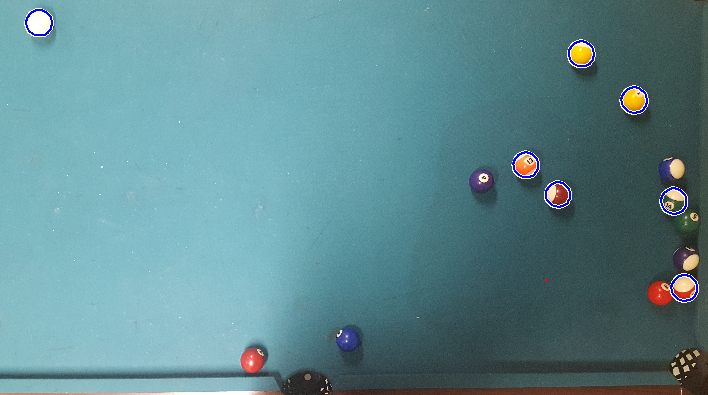
\includegraphics{ballsOnTable.png}
\caption{Results of the VR algorithm.}
\end{figure}~\\

\subsection{Inter-Device Communication}
The system must have a smartphone receive a message wirelessly from the PC and then communicate back an image from the smartphone to the PC.\\\\

This problem can be solved using File Transfer Protocol or the Secure CoPy (SCP) protocol. The request will be sent from the PC to the phone which will then capture an image. Upon completion, the PC will use FTP to receive the photo wirelessly from the computer. Relevant links regarding sources of examples for file transfer from an android to a PC and for file permissions management are provided.\\ 

Android to PC file transfer:\\
http://stackoverflow.com/questions/10417442/client-server-file-transfer-from-android-to-pc-connected-via-socket\\

Hardware to Android file transfer over Wi-Fi:\\
http://stackoverflow.com/questions/20345155/android-receive-and-send-data-through-wifi-connection-to-hardware\\

Using the principles discussed above as well as the tangible examples from the link we are confident we can overcome the problem of device intercommunication.

\subsection{Shot Selection}
Shot selection is likely to be the most challenging aspect of this system from a software perspective. Given a set of possible shot angles, amounts of force, and weighted goals the system would need to simulate a multitude of shots. It is infeasible given the computational time requirements of this system to complete this task using a completely brute force approach.\\

The first piece of the solution to this problem is limiting the granularity of angles to analyze for possible shots. The step size that will be used will be determined as appropriate such that optimal shots are not missed. Furthermore, the step size must be at least the minimum step size of the rotational motor that will aim the end-effector. If it is not possible to take a shot from this angle (e.g. another ball is in the way or the shot is directly into the rails), the algorithm will discard the shot.\\

The algorithm will then simulate taking a shot in that direction at the maximum (100\%) power that the system can safely take. The algorithm will check if the shot causes the cue ball to hit an opponent's ball first, does not hit a ball or sinks the cue ball without hitting a ball. If any of these events are expected to occur, the algorithm will discard the shot.\\

If the shot is not already discarded, certain shot powers will be simulated. This will include an even split somewhere between 4 and 10 of the possible powers (i.e. 25\%/50\%/75\% or 20\%/40\%/60\%/80\%) to be decided based on empirical results later. These shots will be scored based on a number of features such as the robot's balls sunk, opponent balls sunk, if the cue ball was sunk, and so on. The algorithm will go from higher power to lower power. Therefore, if at low power it does not hit a ball, the algorithm can neglect checking lower powers at that shot angle.\\

These logical steps will substantially lower the duration of computation to be made by the algorithm. Our hope is that using this algorithm the duration will be short enough to satisfy the computational time requirement.



\section{Hardware Proof of Concept}
This section will outline the major hardware hurdles that must be overcome in order for this project to be a success. For each case, the concern will be discussed followed by the team's plan on how to overcome that issue.
\subsection{Post-Shot Interference}
In order to adequately strike a ball anywhere on the table the end-effector or striker will be required to enter the active ball area (the theoretical volume at which object inside it may interfere with a moving ball). The end-effector must enter this volume to initiate contact with the ball but must quickly exit it in order to allow the balls to move freely.\\

Our team will address this issue by creating a mechanism that will raise the end-effector soon after the shot using either a rotating or linear actuator. This will be done as quickly as possible without damaging the instruments or requiring human intervention to reset it to its striking position.
\subsection{Machine State Awareness}
When the system moves from one location to another it will keep track of its new location by counting steps. This is why being able to count the number of steps of translational and rotational motors is essential to the success of the project. A difficulty which we may encounter is both the real time tracking of steps and the loss of steps due to disturbances or system error.\\

We will address this issue in several ways. Firstly, the system must be well built in order to minimize the motor's gears slipping or skipping steps. Second, we are estimating that most if not all motors will be stepper motors which have a definite mechanical step rather than servos which rely on other tracking methods. We will have a dedicated system within the $\mu$C software that will track each step carefully in order to avoid inaccuracies. If the system detects a potential miscalculation there will be known checkpoints that the system will use to calibrate the current step. These checkpoints should be frequent enough for the program to reset fairly often. The actual number of checkpoints is based on the accuracy of the motor and structure of the system (i.e. an inaccurate system will require more checkpoints). There will likely be somewhere between 2 and 10 checkpoints depending on the integrity of the motion.
\subsection{Recoil from Shots}
The end-effector will be required to strike at many levels of force in order to score from different positions on the table. Some of the more powerful shots may induce large amounts of recoil in the robotic arm. In order to avoid interfering with the other balls on the table and to avoid damaging the system, the recoil from a shot must be accounted for. Optimally, the system will be built sturdy enough that it can handle this recoil. Failing that, one of the following two options will be used. One is that a real-time control system could be implemented. The control system will invoke a force opposite to the recoil of the system in order to maintain the stability of the system. The other option would be to have some sort of bracing system that "digs in" while a shot is being made.
\subsection{Shot Power Control}
The end-effector will be required to strike at a variable force as determined by the shot selection algorithm. The system must then translate the specified amount of power into the appropriate motion. Most likely, the end-effector will utilize a pneumatic piston to make its shot. In this case, the system will have to be designed in a way that provides as many preset amounts of force as necessary as it can only handle certain fixed values. Another option would be a motor. In that case, the correct voltage will need to be applied to the motor for an appropriate amount of time.\\

\subsection{Ability to Make All Shots}
This concern was briefly addressed in the software section concerning the shot selection algorithm. However, the machine will also be designed in such a way as to minimize the amount of space required to take a shot. For example, a longer end-effector will be able to operate in tighter spaces. In addition, the end-effector will strike at a slight angle in order to allow shots while the cue ball is resting on the rails of the table. These solutions should be sufficient to allow a wide enough range of shots.

\subsection{Sufficient Motor Torque}
Due to the nature of the task, the end-effector is required to have a high range of motion while also being highly precise. The implication of these requirements is that the mechanical build of the robot arm will likely be of considerable weight. Therefore it is pertinent to address minimum motor specifications required to move the machine.\\

The most pressing concern is specifications required to facilitate movement along the length of the table as this will require being able to move the entire weight of the machine.  A liberal estimate of 250 kg for the mass of the robot will be assumed. Some form of slide bearing will aid movement of the machine along the length of the table. An estimate of 0.3 for coefficient of static friction (mu) will be assumed. This is also a very liberal estimate as the coefficient of static friction for slide bearings can vary anywhere from approximately 0.003 to 0.3. Using the mass of the robot and the coefficient of static friction, a force of $250*9.81*0.3 = 735.75$ N is required to move the machine along the length of the table.\\

While 735.75 N is a rather high value, it is not entirely unfeasible. It is possible to purchase two stepper motors rated for 25 N-m stall torque. This translates to 735.75 N of force at roughly a 6.8 cm effective radius (radius to translate motor rotation to linear motion). As it is likely that an even smaller radius for this purpose will be used, 6.8 cm is a perfectly acceptable metric. Furthermore, intelligent planning with regards to the design of the robot arm will result in a total weight much less than 250kg, average quality slide bearings will result in a coefficient of static friction much less than 0.3, and gear ratios can be utilized to increase the torque provided if necessary. These factors will reduce the required stall torque of the motors.\\

An example of a motor of this capability can be found in the following link for around \$200:\\
http://www.omc-stepperonline.com/high-torque-nema-42-cnc-stepper-motor-30nm4248ozin-p-74.html
Furthermore, 
\subsection{Rigid Structure}
A large portion of the system will include rails to provide support for translational motion of the end-effector. As a result, sufficiently rigid bars that span the length of the table must be used. Furthermore all jitter, shaking, or unnecessary motion must be reduced in order to provide stability for the system and avoid inaccuracies in the machine's motion.\\

This will be addressed through the selection of non-flexing materials. These materials will be sturdy and straight at the length required by the design. Additionally, beams can be located along the way to provide additional support as necessary. Finally, the system must be designed to allow minimal jitter space within connections. All mechanical connections must be tight and be able to withstand environmental disturbances. 
\end{document}